\section{Method}

\begin{figure*}[t]
  \centering
  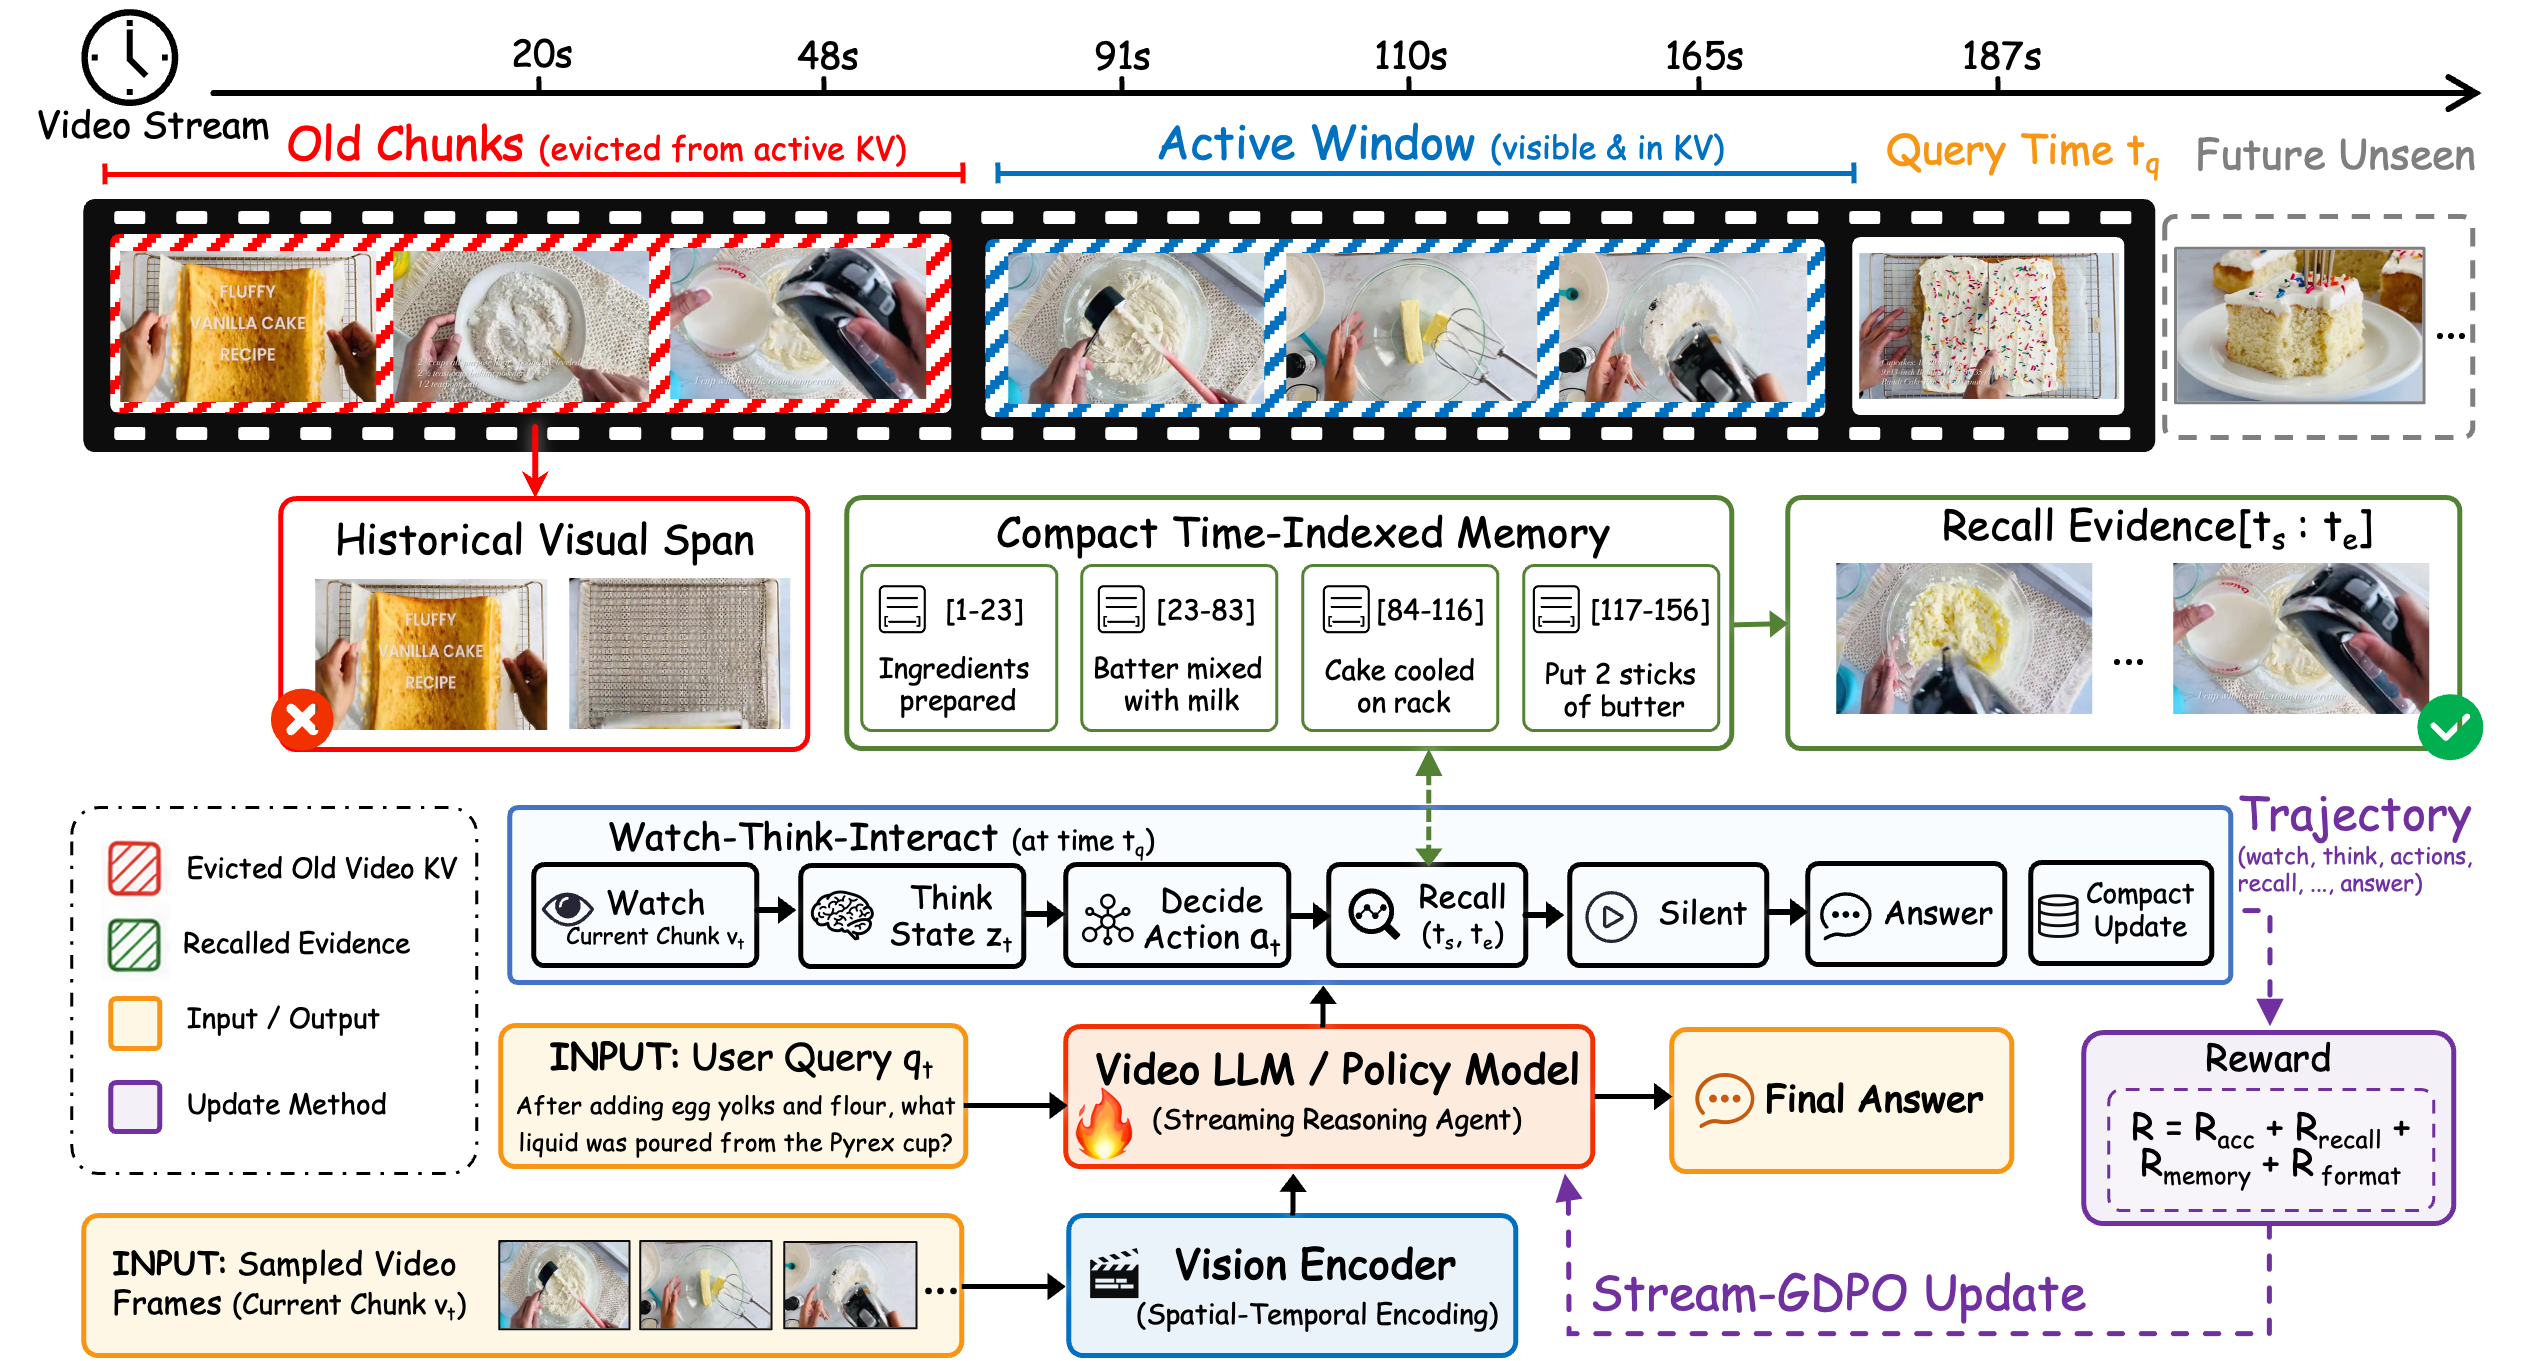
\includegraphics[width=\textwidth]{figures/figure_method_pipeline.png}
  \caption{Overview of Watch-Think-Interact. WTI treats streaming video reasoning as a bounded online loop in which the model watches each incoming chunk, updates a thinking state, and decides whether to stay silent, answer, or recall a past interval. Compact time-indexed memory carries history beyond the active window, and Stream-GDPO optimizes the resulting interaction trajectory.}
  \label{fig:method_overview}
\end{figure*}

\subsection{Problem Definition}

We study online multi-turn streaming video reasoning.
A video arrives as an ordered stream of chunks:
\begin{equation}
  V=(c_1,\ldots,c_T).
\end{equation}
At step \(t\), the model can condition only on the observed prefix \(c_{\le t}\), so future chunks are unavailable.

The same stream may contain multiple timed user questions:
\begin{equation}
  \mathcal Q=\{(q_r,\tau_r,\alpha_r)\}_{r=1}^{R}.
\end{equation}
Here \(\tau_r\) is the question timestamp and \(\alpha_r\) is the answer timestamp used for data construction and evaluation.
Questions are ordered by timestamp, \(1\le\tau_1\le\cdots\le\tau_R\), and each answer timestamp satisfies \(\tau_r\le\alpha_r\le T\).
The answer timestamp marks when sufficient visual evidence is available, but it is not given to the model at inference time.
For each question, the model outputs an answer \(\hat y_r\) at response time \(\hat t_r\ge\tau_r\).
The goal is to produce a visually grounded answer at a valid response time.
A response before \(\alpha_r\) is not valid under strict streaming causality, while a valid response should be supported by \(c_{\le \hat t_r}\).

\subsection{Watch-Think-Interact Framework}

Given the streaming problem above, we instantiate the model as an online multimodal agent.
At step \(t\), the agent receives the newly arrived chunk \(c_t\) and acts under the following state:
\begin{equation}
  s_t=(c_t,W_t,M_t,Q_t,H_t).
\end{equation}
Here \(W_t\) is the active visual window, \(M_t\) is the compact textual memory, \(Q_t\) is the active question set, and \(H_t\) is the interaction history.
Historical evidence outside the active window is carried by time-indexed memory lines with evidence boundaries, rather than being fully inserted into the model context at every step.

Each step combines a streaming thinking update with an interaction decision.
The model first emits a short update \(z_t\) and then selects one interaction action:
\begin{equation}
  \begin{aligned}
  a_t\in\mathcal A_{\mathrm{int}}
  =\{&\mathrm{silence},\mathrm{response}(q_r,y),\\
     &\mathrm{recall}(\tau_s,\tau_e)\}.
  \end{aligned}
\end{equation}
The action \(\mathrm{silence}\) delays output, \(\mathrm{response}\) commits an answer to the current question, and \(\mathrm{recall}\) requests evidence from a previously observed interval.

A recall action is valid only when \(\tau_s\le\tau_e<t\).
The environment returns evidence from this interval as an observation, which is added to the context for the subsequent assistant decision.

At a memory boundary \(b\), let \(Z_b\) collect the streaming records since the previous boundary.
The model rewrites the pre-update memory into a new compact memory:
\begin{equation}
  M_{\mathrm{post}}=\operatorname{Compact}_{\theta}(M_{\mathrm{pre}},Z_b).
\end{equation}
The memory size is bounded by \(\lvert M_{\mathrm{post}}\rvert\le B_M\).
Each memory line stores a concise semantic note with its video time range, providing a structured index for later recall.
This keeps the resident state compact while preserving time-indexed entries for later recall-based evidence inspection.

Together, these operations define a bounded online loop in which the agent consumes each chunk once, maintains time-indexed memory beyond the active window, and recalls past intervals only when needed for the current decision at that step.

\subsection{Masked Supervised Fine-Tuning}

The supervised stage aligns training with the bounded context used by the online agent~\citep{streamingvlm2026}.
At step \(t\), SFT uses the same online state as inference, while the dense visual context is limited to the recent window
\begin{equation}
  W_t=\{c_{\max(1,t-K_v+1)},\ldots,c_t\},
\end{equation}
where \(K_v\) is the visual window size.
Compact memory \(M_t\), active questions \(Q_t\), and interaction history \(H_t\) provide the textual state, so each target is conditioned on the state available at inference rather than on a full video prefix that the model will not retain.

For each stream, we serialize stream inputs, assistant outputs, and environment observations in temporal order, so each assistant target is trained under the online prefix available at its stream step.
To train autoregressively on this sequence, we apply a stream-causal mask under which each assistant token can attend only to tokens available from earlier stream steps and to its causal prefix.

Environment outputs are used only as conditioning context for later assistant targets.
Accordingly, a token-wise label mask limits supervised loss to assistant-generated tokens.
Because action targets are sparse and state-update spans are longer, a single token average can overemphasize frequent or long targets.
We average valid token losses separately for the action and state-update groups, denoted by \(\bar\ell_{\mathrm{act}}\) and \(\bar\ell_{\mathrm{state}}\).
The action group contains silence, response, and recall targets, while the state-update group contains thinking and compact-memory targets.
The bucket-weighted SFT objective is
\begin{equation}
  \mathcal L_{\mathrm{SFT}}(\theta)
  =
  \lambda_{\mathrm{act}}\bar\ell_{\mathrm{act}}
  +
  \lambda_{\mathrm{state}}\bar\ell_{\mathrm{state}}.
\end{equation}
This stage trains the bounded-context protocol.

\begin{table*}[t]
  \centering
  \footnotesize
  \renewcommand{\arraystretch}{1.18}
  \setlength{\tabcolsep}{4.5pt}
  \resizebox{\textwidth}{!}{
  \begin{tabular}{l|cccccc|c|ccc|c|ccc|c|c}
    \hline
    \multicolumn{1}{c|}{\multirow{2}{*}{\textbf{Model}}} & \multicolumn{7}{c|}{\textbf{Real-Time}} & \multicolumn{4}{c|}{\textbf{Backward}} & \multicolumn{4}{c|}{\textbf{Forward}} & \textbf{Overall} \\
    \cline{2-17}
    & \textbf{OCR} & \textbf{ACR} & \textbf{ATR} & \textbf{STU} & \textbf{FPD} & \textbf{OJR} & \textbf{Avg.} & \textbf{EPM} & \textbf{ASI} & \textbf{HLD} & \textbf{Avg.} & \textbf{REC} & \textbf{SSR} & \textbf{CRR} & \textbf{Avg.} & \textbf{Avg.} \\
    \hline
    \rowcolor{softred}
    \multicolumn{17}{c}{\textbf{Proprietary models}} \\
    \hline
    GPT-4o & 69.8 & 64.2 & 71.6 & 51.1 & 70.3 & 59.8 & 64.5 & 57.9 & 75.7 & 48.7 & 60.8 & 27.6 & 73.2 & 59.4 & 53.4 & 59.5 \\
    Gemini-1.5-Pro & 85.9 & 67.0 & 79.3 & 58.4 & 63.4 & 62.0 & 69.3 & 58.6 & 76.4 & 52.6 & 62.5 & 35.5 & 74.2 & 61.7 & 57.2 & 63.0 \\
    \hline
    \rowcolor{softorange}
    \multicolumn{17}{c}{\textbf{Open-source offline models}} \\
    \hline
    LongVU-7B & 53.7 & 53.2 & 62.9 & 47.8 & 68.3 & 59.8 & 57.6 & 40.7 & 59.5 & 4.8 & 35.0 & 12.2 & 69.5 & 60.8 & 47.5 & 46.7 \\
    LLaVA-OV-7B & 66.4 & 57.8 & 73.3 & 53.4 & 71.3 & 62.0 & 64.0 & 54.2 & 55.4 & 21.5 & 43.7 & 25.6 & 67.1 & 58.8 & 50.5 & 52.7 \\
    LLaVA-Video-7B & 69.1 & 58.7 & 68.8 & 49.4 & 74.3 & 59.8 & 63.5 & 56.2 & 57.4 & 7.5 & 40.4 & 34.1 & 70.0 & 60.4 & 54.8 & 52.9 \\
    LLaVA-NeXT-Video-7B & 69.8 & 59.6 & 66.4 & 50.6 & 72.3 & 61.4 & 63.3 & 51.2 & 64.2 & 9.7 & 41.7 & 34.1 & 67.6 & 60.8 & 54.2 & 53.1 \\
    Qwen2.5-VL-7B & 67.8 & 55.1 & 67.2 & 42.1 & 66.3 & 60.9 & 58.9 & 51.5 & 58.8 & 32.2 & 47.5 & 34.1 & 67.6 & 60.8 & 63.6 & 57.3 \\
    Qwen3-VL-8B & 75.2 & 58.7 & 72.4 & 57.3 & 70.3 & 59.2 & 64.8 & 56.6 & 69.6 & 38.7 & 54.4 & 38.8 & 67.6 & 52.5 & 63.5 & 61.4 \\
    \hline
    \rowcolor{softgreen}
    \multicolumn{17}{c}{\textbf{Open-source streaming models}} \\
    \hline
    Flash-VStream-7B & 24.2 & 29.4 & 28.5 & 33.7 & 25.7 & 28.8 & 28.4 & 39.1 & 37.2 & 5.9 & 27.4 & 8.0 & 67.3 & 60.0 & 45.1 & 33.6 \\
    Dispider-7B & 57.7 & 49.5 & 62.1 & 44.9 & 61.4 & 51.6 & 54.6 & 48.5 & 55.4 & 4.3 & 36.1 & 18.1 & 37.4 & 48.8 & 34.7 & 41.8 \\
    TimeChat-Online-7B & 74.5 & 48.6 & 68.1 & 48.3 & 69.3 & 59.8 & 61.4 & 56.9 & 64.9 & 11.8 & 44.5 & 31.8 & 38.5 & 40.0 & 36.8 & 47.6 \\
    StreamForest-7B & 68.5 & 53.2 & 71.6 & 47.8 & 65.4 & 60.9 & 61.2 & 58.9 & 64.9 & 32.3 & 52.0 & 32.8 & 70.6 & 57.1 & 53.5 & 55.6 \\
    Streamo-7B & 77.2 & 66.1 & 76.7 & 45.5 & 66.3 & 72.8 & 67.4 & 55.6 & 58.1 & 33.9 & 49.2 & 30.8 & 57.6 & \textbf{82.5} & 57.0 & 57.9 \\
    ViSpeak-7B & 75.2 & 58.7 & 71.6 & 51.1 & 74.3 & 66.9 & 66.3 & 59.9 & 48.7 & 64.0 & 57.5 & 33.8 & 68.5 & 60.4 & 54.3 & 61.1 \\
    StreamBridge-7B & 84.6 & 71.6 & 74.1 & 49.4 & 75.3 & 72.8 & 71.3 & \textbf{67.7} & 57.4 & 79.0 & \textbf{68.1} & 19.2 & 64.3 & 61.7 & 48.4 & 62.6 \\
    \rowcolor{softblue}
    WTI-8B (Ours) & \textbf{90.6} & \textbf{76.2} & \textbf{78.5} & \textbf{66.9} & \textbf{76.2} & \textbf{75.5} & \textbf{76.9} & 67.0 & \textbf{74.3} & \textbf{82.8} & \textbf{73.4} & 42.2 & \textbf{73.1} & 77.1 & \textbf{70.0} & \textbf{73.6} \\
    \hline
  \end{tabular}}
  \caption{Results on OVO-Bench. Scores are grouped by Real-Time, Backward, and Forward tasks; Avg. reports group averages and Overall reports the benchmark average.}
  \label{tab:ovobench_main}
\end{table*}


\subsection{Stream-GDPO Reinforcement Learning}

After masked SFT, Stream-GDPO trains the policy in the same chunk-level environment used at inference.
Each rollout contains one video stream with one or more timed questions.
The policy acts from the current online state, while chunk arrival and recall returns are treated as environment feedback.

Stream-GDPO uses question-level rewards for answer outcome, format validity, and recall use, together with a rollout-level compact-memory reward.
The answer outcome is computed by a form-aware verifier
\begin{equation}
  R_{\mathrm{out}}^{i,q}
  =
  \max_{y\in\mathcal Y_q}
  \mathbb I\!\left(\operatorname{match}(\hat y_{i,q},y)\right),
\end{equation}
where \(\mathcal Y_q\) is the valid-answer set and timing validity with respect to \(\alpha_q\) is included in the verifier.
\(R_{\mathrm{fmt}}\) checks whether actions follow the streaming protocol.

Let \(u_{i,q}\) indicate whether rollout \(i\) recalls evidence for \(q\), and let \(\mathcal Q_{\mathrm{BT}}\) denote Backward Tracing questions.
The recall-tool reward is
\begin{equation}
  R_{\mathrm{tool}}^{i,q}
  =
  \mathbb I(q\in\mathcal Q_{\mathrm{BT}})
  \mathbb I(u_{i,q}=1).
\end{equation}

For compact-memory writing, the reward measures whether an update improves the stream memory.
Let \(S_{\mathrm{time}}(M)\) score the time indexing quality of memory \(M\), and let \(S_{\mathrm{keep}}(M)\) score its retention of salient stream facts.
For an update \(M_{\mathrm{pre}}^i\to M_{\mathrm{post}}^i\), we define
\begin{equation}
  \begin{aligned}
  R_{\mathrm{mem}}^i
  =
  \frac{1}{2}\Big[
  &S_{\mathrm{time}}(M_{\mathrm{post}}^i)-S_{\mathrm{time}}(M_{\mathrm{pre}}^i)\\
  &+S_{\mathrm{keep}}(M_{\mathrm{post}}^i)-S_{\mathrm{keep}}(M_{\mathrm{pre}}^i)
  \Big].
  \end{aligned}
\end{equation}
Thus, compact-memory quality is rewarded as an update difference, not as an absolute score.

Let \(R_{\mathrm{out}}^i\) and \(R_{\mathrm{fmt}}^i\) denote the averaged outcome and format rewards over questions in rollout \(i\).
Let \(R_{\mathrm{tool}}^i\) denote the averaged recall-tool reward.
The rollout reward combines the four terms
\begin{equation}
  \begin{aligned}
  R_i={}&
  R_{\mathrm{out}}^i
  +R_{\mathrm{fmt}}^i\\
  &+\lambda_{\mathrm{tool}}R_{\mathrm{tool}}^i
  +\lambda_{\mathrm{mem}}R_{\mathrm{mem}}^i.
  \end{aligned}
\end{equation}
The compact-memory reward remains a rollout-level term because it is not question-specific.

Within each rollout group, Stream-GDPO normalizes the rollout rewards \(\{R_i\}\) to obtain a group-relative trajectory advantage \(A_i\).
We assign \(A_i\) to the assistant action turns selected for policy optimization from the same rollout.
The policy is optimized with the clipped objective
\begin{equation}
  \mathcal J_{\mathrm{GDPO}}(\theta)
  =
  \mathbb E_{i,j}\!\left[
  \min(\rho_{i,j}A_i,\tilde\rho_{i,j}A_i)
  -\beta D_{i,j}
  \right].
\end{equation}
\(\tilde\rho_{i,j}\) clips \(\rho_{i,j}\) to \([1-\epsilon,1+\epsilon]\), \(\rho_{i,j}\) is the action-turn probability ratio between \(\pi_\theta\) and \(\pi_{\theta_{\mathrm{old}}}\), and \(D_{i,j}\) is the KL penalty to the reference policy at state \(s_{i,j}\).
We minimize \(\mathcal L_{\mathrm{GDPO}}=-\mathcal J_{\mathrm{GDPO}}\).
This keeps credit assignment at the trajectory level, without estimating separate turn- or token-level advantages.

\section{WTI-82K}
\label{sec:data}

\begin{figure*}[t]
  \centering
  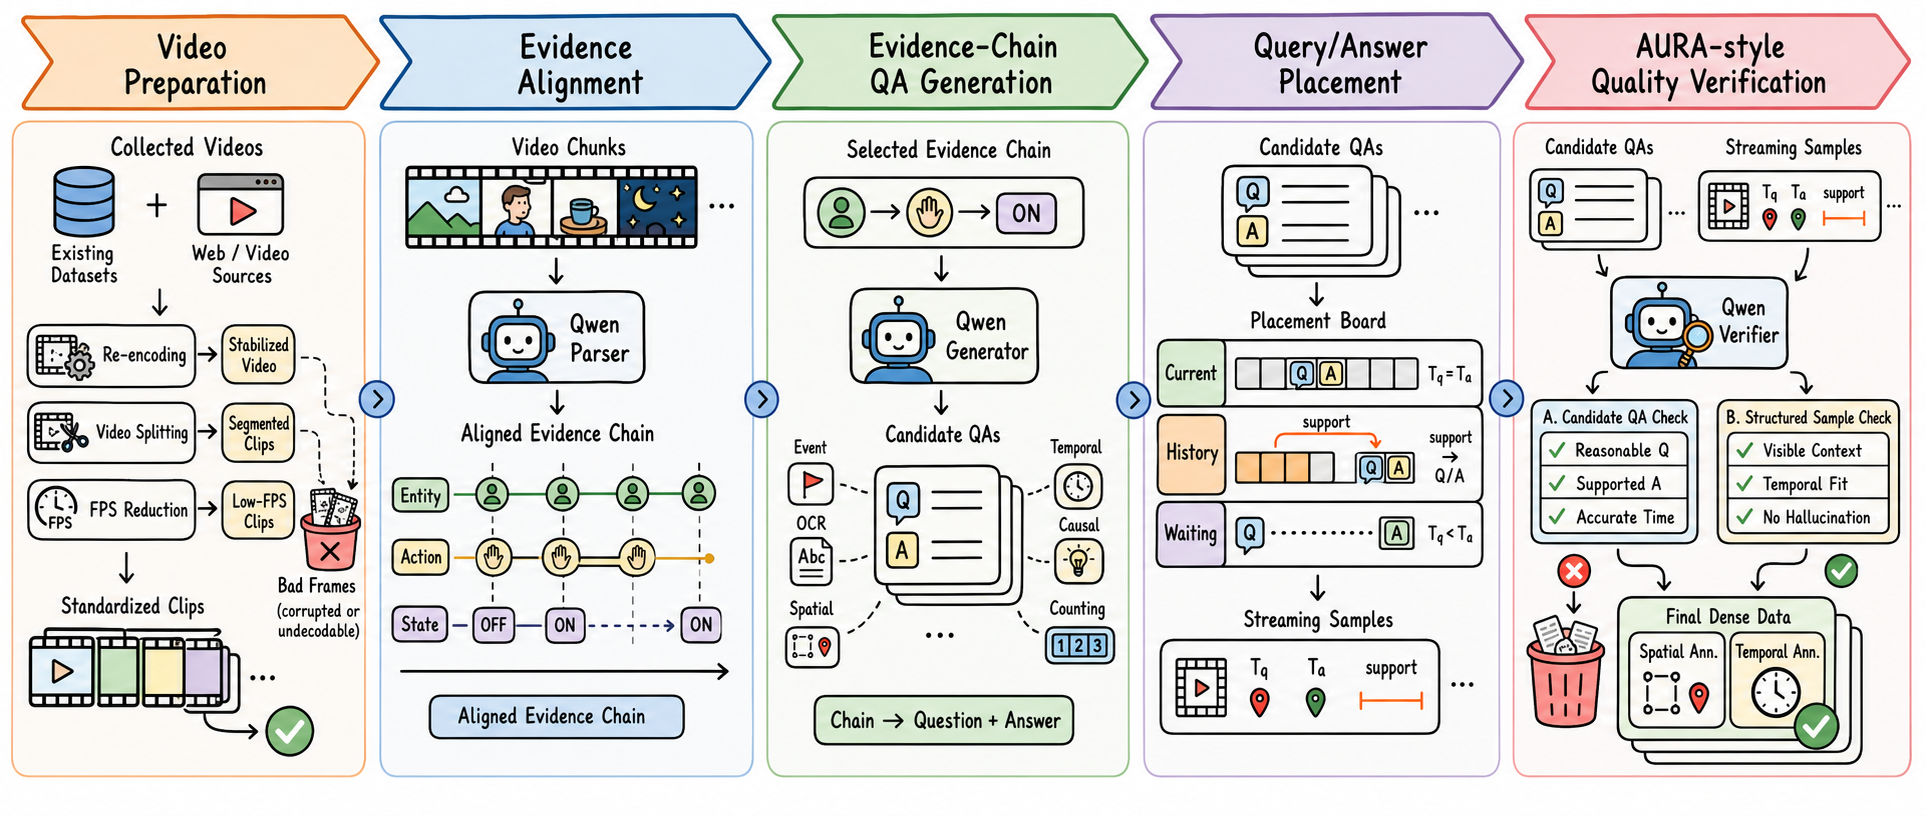
\includegraphics[width=\textwidth]{figures/figure_data_pipeline.png}
  \caption{WTI-82K construction pipeline. WTI-82K converts videos into streaming-causal trajectories by standardizing clips, aligning chunk-level evidence chains, generating evidence-grounded QAs, placing query and answerable times, and verifying causal support. The resulting samples cover Real-Time, Backward Tracing, and Proactive interactions used to train WTI under the same timing constraints as inference.}
  \label{fig:data_pipeline}
\end{figure*}

Prior online video benchmarks and streaming instruction datasets define timestamped queries, multi-turn interaction, proactive responses, and streaming task annotations~\citep{ovobench2025,svbench2025,streambridge2025,streamo2026}.
Building on this setting, we construct WTI-82K, a time-aware dataset for long-horizon multi-turn streaming video reasoning.
It contains 82,335 finalized questions in 4,812 streaming trajectories.
Each sample aligns video chunks, supporting evidence intervals, query time, earliest answerable moment, and the causal context available at that moment.
As shown in Figure~\ref{fig:data_pipeline}, our pipeline extracts temporal evidence, generates evidence-grounded questions, places each query and answerable moment on the streaming timeline, and verifies causal consistency before retention.

\paragraph{Temporal evidence extraction.}
We first filter videos for clear visual content and temporally locatable events.
For each retained video, we extract chunk-level evidence and link facts that persist or change across chunks.
This yields minimal supporting intervals for evidence-chain selection and time-anchored question generation.

\paragraph{Candidate question generation.}
Given the aligned evidence, we use Qwen3.5-397B to generate questions and reference answers from local facts and cross-chunk evidence chains.
The candidates cover immediate perception, historical evidence, temporal progression, and proactive interaction, so each trajectory includes both current-prefix questions and questions requiring long-range state maintenance.

\paragraph{Query-time and answer-time placement.}
Following timestamped online-video protocols~\citep{ovobench2025,svbench2025,streambridge2025}, we then convert each candidate into a streaming sample by assigning a query timestamp and an answerable timestamp based on its supporting evidence interval.
Real-Time samples are answerable at the query time from the current visible prefix.
Backward Tracing samples are also answerable at the query time, but their supporting evidence lies in previously observed chunks and therefore tests history maintenance and recall.
Proactive samples are not answerable when the query appears and require the model to wait until the earliest answerable moment, when decisive future evidence has arrived.
We retain a sample only if its answer is grounded in the causal context available at the answerable moment.
Appendix~\ref{app:data_stats} reports the data statistics and question distribution in detail.
